
%%%%%%%%%%%%%%%%%%
\chapter{Nonparametric and Semiparametric Models}
\section{Nonparametric Regression Models: Introduction}
Consider a setting where we observe the data $(y_i,x_i)$ which is i.i.d. and drawn from a DGP $P_0(y|x)$. Unlike in the parametric setup, we are interested in backing out the whole or part of the data generating process $P_0(y|x)$ \textbf{without any modeling assumptions}. In essence, we are interested in an estimation problem involving an unknown function. This approach is called a \textbf{nonparametric} approach. We normally use nonparametric approach to conduct a diagnostic checking of an estimated parametric model, to conveniently display key features of the dataset, and to conduct an inference under very weak assumptions. \par
For discrete-valued $Y$ and $X$, this is relatively easy. We can back out the data generating process of interest
\[
\hat{P}(y\in A| x\in B)=\frac{n^{-1}\sum_{i=1}^n1(y_i\in A, x_i\in B) }{n^{-1}\sum_{i=1}^n1(x_i\in B)}
\]
Provided that $P_0(x\in B)\neq 0$, then the above estimator converges to the true $P_0(y|x)$ as $n\to\infty$.
\par
When we are working with continuous variables to get an estimate of $P_0(Y\leq y|x)$, one way we could approach is to define $A$ in the above example as $A\equiv (-\infty, y], B\equiv[x-\epsilon, x+\epsilon]$ and use $\lim_{\epsilon\to0}\hat{P}(A|B)$ to back out the DGP. This can be problematic when we have too many dimensions of $X$ (and by too many, the number required for this to happen is not that large). Therefore, the method to conduct nonparametric estimation in this context is kernel density function approach. 
\section{Kernel Density Estimation}
Consider the problem of estimating the probability density function $f(x)$ of a random scalar variable $X$ at $X=x$. We are putting a minimal number of restriction on what $f(x)$ could be. Let $\{X_1,...,X_n\}$ be a random sample of $X$. If $f$ is a smooth function, we can approximate $f$ by
\[
f(x)\simeq \frac{\int_{x-h}^{x+h}f(u)du}{2h}
\]
for a small $h$ (which will later be our bandwith). The numerator on the right hand side can be estimated using a sample analogue of the following form
\[
\frac{1}{n}\sum_{i=1}^n 1\{x-h\leq X_i \leq x+h \}
\]
Combining the two expressions, we can approximate $f(x)$ with
\footnotesize{\begin{align*}
\hat{f}(x)&=\frac{n^{-1}\sum_{i=1}^n 1[x-h\leq X_i \leq x+h]}{2h} \\
&=\frac{1}{2nh}\sum_{i=1}^n 1[x-h\leq X_i \leq x+h]\\
&=\frac{1}{nh}\sum_{i=1}^n \frac{1}{2}1\left[\left|\frac{x-X_i}{h}\right| \leq 1\right]\\
&=\frac{1}{nh}\sum_{i=1}^n K\left(\frac{x-X_i}{h}\right)\\
&=\frac{1}{n}\sum_{i=1}^n K_h(x-X_i)
\end{align*}}\normalsize
where $K(u)=\frac{1}{2}1(|u|\leq 1)$ and $K_h = \frac{1}{h}K\left(\frac{\cdot}{h}\right)$. In general, $K(\cdot)$ is a \textbf{kernel density estimator}. Specifically for this example, I have used a uniform kernel. \par
As for the type of kernel density estimators, there can be many. The requirements are that $K$ is a real-to-real function, positive and smooth and integrates to 1 on its support. For instance, you can use a Gaussian Kernel, $K=\phi$ or an Epanechinkov kernel, defined as $K(u)=\frac{3}{4}\max\{1-u^2,0\}$. However, the selection of $K$ does not matter in most cases. 
\section{Choice of the bandwidth $h$}
While we may have some freedom in choosing $K$, same cannot be said for the bandwidth $h$. This is because our choice of $h$ directly affects the trade-off between the bias and the variance. To see this.
\footnotesize{\begin{align*}
E[\hat{f}(x)]&=E\left[\frac{1}{nh}\sum_{i=1}^n K\left(\frac{x-X_i}{h}\right)\right]\\
&=\frac{1}{h}\int_{-\infty}^\infty K\left(\frac{x-s}{h}\right)f(s)ds\\
&=-\frac{1}{h}\int_{-\infty}^\infty K(t)f(x-ht)(-hdt) \ (\because \frac{x-s}{h}=t \ \text{transformation})\\
&=\int_{-\infty}^\infty K(t)f(x-ht)dt\\
&=\int_{-\infty}^\infty K(t)\left[f(x)-f'(x)ht + \frac{f''(x)h^2t^2}{2}+o(h^2)\right]dt\\
&=f(x)-0+\frac{1}{2}\int_{-\infty}^\infty K(t)h^2t^2f''(x)dt + o(h^2)
\end{align*}}\normalsize
Where $\int_{-\infty}^\infty K(t)dt=1$ justifies $f(x)$ and $\int_{-\infty}^\infty tK(t)dt=0$ (since kernel is symmetric around 0) justifies second term in the last line being 0.\footnote{In the lecture slides, $O(h^2)=\frac{f''(x)h^2t^2}{2}+o(h^2)$} As such, the bias is captured by 
\[
E[\hat{f}(x)]-f(x)=\frac{1}{2}\int_{-\infty}^\infty K(t)h^2t^2f''(x)dt
\]
Therefore, smaller bandwidth $h$ reduces the bias.\par
 However, for variance, we have
 \footnotesize{\begin{align*}
Var[\hat{f}(x)]&=E[\hat{f}^2(x)]-(E[\hat{f}(x)])^2\\ 
&=E\left[\frac{1}{n^2h^2}\left(\sum_{i=1}^nK\left(\frac{x-X_i}{h}\right)\right)^2\right]-(E[\hat{f}(x)])^2\\
&=E\left[\frac{1}{n^2h^2}\left(\sum_{i=1}^nK^2\left(\frac{x-X_i}{h}\right)+2\sum_{i<j} K\left(\frac{x-X_i}{h}\right)K\left(\frac{x-X_j}{h}\right)\right)\right]-(E[\hat{f}(x)])^2\\
&=\frac{1}{nh^2}\int_{-\infty}^\infty K^2\left(\frac{x-s}{h}\right)f(s)ds+\frac{n(n-1)}{n^2h^2}\left(\int_{-\infty}^\infty K\left(\frac{x-s}{h}\right)f(s)ds\right)^2-\frac{1}{h^2}\left(\int_{-\infty}^\infty K\left(\frac{x-s}{h}\right)f(s)ds\right)^2
 \end{align*}}\normalsize
 Then, we use the Taylor expansion and the variable transformation $\frac{x-s}{h}=t$ on each of the terms. As a result, we can show that the first term can be written
 \footnotesize{\[
 \frac{1}{nh^2}\int_{-\infty}^\infty K^2\left(\frac{x-s}{h}\right)f(s)ds=\frac{1}{nh}\int_{-\infty}^\infty K^2(t)f(x-ht)dt\simeq \frac{1}{nh}\int_{-\infty}^\infty K^2(t)f(x)dt
 \]}\normalsize
 so that $\frac{1}{nh}\int_{-\infty}^\infty K^2(t)f(x)dt$ is the leading term. The other two terms will be cancelled out as $n\to\infty$, as 
 \footnotesize{\[
\left( \frac{n(n-1)}{n^2h^2}-\frac{1}{h^2}\right)\left(\int_{-\infty}^\infty K\left(\frac{x-s}{h}\right)f(s)ds\right)^2 =-\frac{1}{nh^2} \left(\int_{-\infty}^\infty K\left(\frac{x-s}{h}\right)f(s)ds\right)^2
 \]}\normalsize
  Since the first term can be written as $O\left(\frac{1}{nh}\right)$, smaller $h$ increases the variance.  \par
 So what determines the optimal $h$? The answer is the $h$ that minimizes the loss function, or asymptotic mean integrated squared error (AMISE), defined as
 \[
 \int E(\hat{f}(x)-f(x))^2dx
 \]
 where the bias-variance decomposition of MSE kicks in as follows
 \small{\begin{align*}
 E[(\hat{f}(x)-f(x))^2] &=E[(\hat{f}(x)-E(\hat{f}(x))+E(\hat{f}(x))-f(x))^2]\\
 &=E[(\hat{f}(x)-E(\hat{f}(x)))^2+(E(\hat{f}(x))-f(x))^2 +2(\hat{f}(x)-E(\hat{f}(x)))(E(\hat{f}(x))-f(x))]\\
 &=E[(\hat{f}(x)-E(\hat{f}(x)))^2]+E[(E(\hat{f}(x))-f(x))^2]\\
 &=\text{Variance}+\text{Bias}^2
 \end{align*}}\normalsize\par
 From the discussion about the bias and variance above, we can write
 \begin{align*}
 \text{Variance}+\text{Bias}^2=\frac{1}{nh}\int_{-\infty}^\infty K^2(t)f(x)dt+\frac{h^4}{4}(f''(x))^2\left(\int_{-\infty}^\infty K(t)t^2dt\right)^2
 \end{align*}
 Thus, the final version of AMISE can be written as
 \[
 \int(\text{Variance}+\text{Bias}^2)dx=\frac{1}{nh}\int_{-\infty}^\infty K^2(t)dt+\frac{h^4}{4}\int_{-\infty}^\infty(f''(x))^2\left(\int_{-\infty}^\infty K(t)t^2dt\right)^2 dx
 \]
 For a shorthand notation, we can write $A=\frac{1}{4}\int_{-\infty}^\infty(f''(x))^2\left(\int_{-\infty}^\infty K(t)t^2dt\right)^2 dx$, $B=\int_{-\infty}^\infty K^2(t)dt$ to get
 \[
 AMISE =Ah^4+\frac{B}{nh}
 \]
 Then, the minimization problem becomes $\min_h AMISE$. Therefore, we find $h$ satisfying
 \[
 4Ah^3-Bn^{-1}h^{-2}=0\iff h^5=\frac{B}{4An} \iff h=\left(\frac{B}{4An}\right)^{1/5}
 \]
 In this framework, the bias and standard errors are both in $n^{-2/5}$ and AMISE will be in $n^{-4/5}$. Therefore, we may not have a CAN estimator at $n^{-1/2}$, which is what is normally the case. Even bigger problem arises from $\int f''(x)dx$ term in $A$, as we are not sure of $f(x)$ to begin with, we do not know what $f''(x)$ would be. There are several ways to deal with this.
 \begin{itemize}
 \item\textbf{Silverman's Rule of Thumb}: If $K$ is a normal kernel and $f(x)$ is normal with some variance $\sigma^2$, Silverman's rule of thumb implies the benchmark
 \[
 h=1.06\sigma n^{-1/5}
 \]
 where $\sigma$ can be replaced with sample standard deviation $s$. For a more robust version, we can use
 \[
 h=0.9 \min\{s,IQ/1.34\}n^{-1/5}
 \]
 where $IQ$ is an interquartile distance. 
 \item\textbf{Cross-validation}: This method is similar to the original method in the sense that we are selecting some $h$ that minimizes certain criterion function, $CV(h)$. In this case, we are using a leave-one-out estimator. This is usually calculated as
 \[
 \hat{f}_{-i}(x) = \frac{1}{nh}\sum_{j\neq i}K\left(\frac{x-x_j}{h}\right)
 \]
 for every observation $i$. This is computationally burdensome and the resulting $h$ converges very slowly ($n^{-1/10}$). 
  \item\textbf{Local Bandwidth}: You may care only about $f(x)$ at a given point. The key idea is to make $h$ larger in a low density area, as low density could imply larger spread in the distribution of $f(x)$. Making $h$ larger would decrease variance. In a wiggly region, it is better to take $h$ smaller. The distribution can take many values and bias can be problematic. Reducing $h$ would minimize worries about biases. 
 \end{itemize}
 \begin{mdframed}[backgroundcolor=yellow!5]
\begin{comment}[So why worry about bandwidth to begin with?]
If $h$ is smaller than the optimal bandwidth length, we say that there is an \textbf{undersmoothing}. If otherwise, we say \textbf{oversmoothing} is present. When there is an undersmoothing, there are too much more detail than necessary and in some areas, leading to computational difficulty. When there is an oversmoothing, we risk masking some important detail about the distribution of $f(x)$. We may end up with a normal distribution even if it really is not. \par
Below is a figure that I borrowed from a statistics lecture note from CMU.\footnote{https://www.stat.cmu.edu/~larry/=sml/densityestimation.pdf}
\begin{figure}[H]
\centering
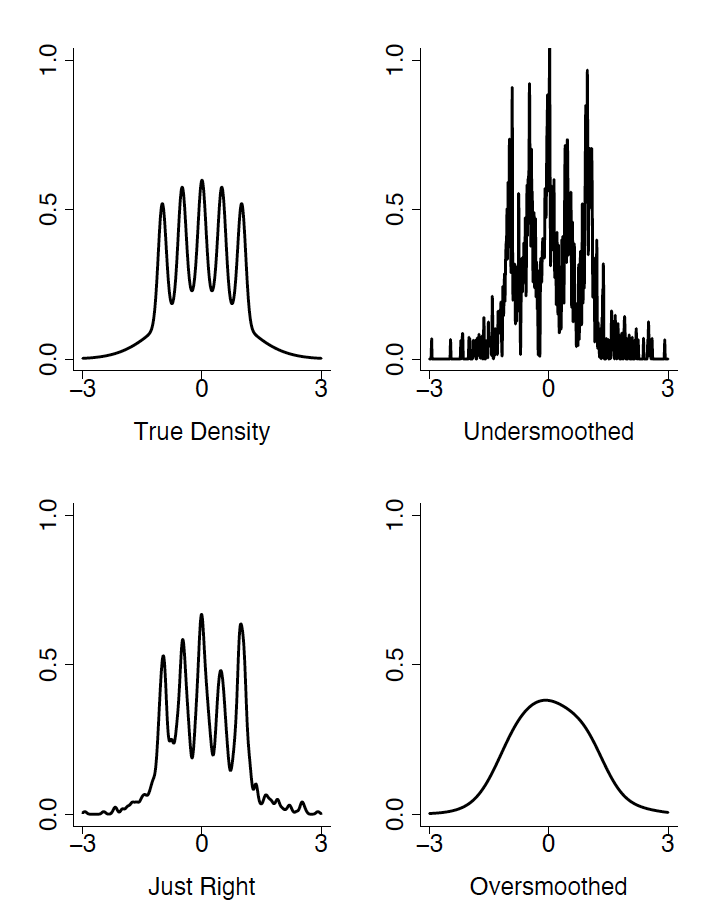
\includegraphics[width=0.5\textwidth, keepaspectratio]{smoothing.png}
\end{figure}
\end{comment}
\end{mdframed}
 \section{Curse of Dimensionality}
 Now assume that $x$ is not necessarily a scalar, but of dimension $d$. Then we can use a $d$-dimensional kernel $K$ and estimate $f(x)$ with
 \[
 \hat{f}(x)= \frac{1}{nh^d}\sum_{i=1}^nK\left(\frac{x-x_i}{h}\right)
 \]
 where $K$ can be a $d$-product of a uni-dimensional kernels. In addition, we are not necessarily confined to using a same bandwith for all $d$ kernels. For instance, if you know that the variance of $x_1$ is larger than $x_2$ you may want higher $h_1$ relative to $h_2$ to avoid variance of the kernel density estimator for the first covariate from being too large. We may want to sphericize if the kernel estimators are correlated. \par
 A bigger concern has to do with the computation cost from using a large $d$. This is what \textbf{curse of dimensionality} refers to. If we return to calculating $E[\hat{f}(x)^2]$ term in the variance component of AMISE, 
 \footnotesize{\begin{align*}
 E[\hat{f}(x)^2]&=E\left[\frac{1}{n^2h^{2d}}\left(\sum_{i=1}^nK\left(\frac{x-X_i}{h}\right)\right)^2\right]\\
 &=E\left[\frac{1}{n^2h^{2d}}\left(\sum_{i=1}^nK^2\left(\frac{x-X_i}{h}\right)+2\sum_{i<j} K\left(\frac{x-X_i}{h}\right)K\left(\frac{x-X_j}{h}\right)\right)\right]\\
 &=\frac{1}{nh^{2d}}\int_{-\infty}^\infty K^2\left(\frac{x-s}{h}\right)f(s)ds+\frac{n(n-1)}{n^2h^{2d}}\left(\int_{-\infty}^\infty K\left(\frac{x-s}{h}\right)f(s)ds\right)^2
 \end{align*}}\normalsize
 Again, the leading term is
 \[
\frac{1}{nh^{2d}}\int_{-\infty}^\infty K^2\left(\frac{x-s}{h}\right)f(s)ds \simeq \frac{1}{nh^d}\int K^2(t)f(x-ht)dt
 \]
 since $s$ is actually $d$-dimensional. Thus, the variance is now $O\left(\frac{1}{nh^d}\right)$. What this means is that $AMISE=Ah^4+\frac{B}{nh^d}$ and the optimal $h$ is solved as
 \[
 h=\left(\frac{Bd}{4An}\right)^{1/(4+d)}
 \]
 Thus, $h$ will be in $n^{-\frac{1}{4+d}}$ and convergence occurs in $n^{-\frac{2}{4+d}}$ - at an even slower rate that when $d=1$, which was already slower than parametric convergence rate. AMISE would be in order $n^{-\frac{4}{4+d}}$\par
 
 \section{Local Constant and Polynomial Estimation}
 Given the data $(y_i,x_i)$, we are attempting to capture $E[g(y,x)|x]=m(x)$ for some $g(y,x)$. For instance, we can attempt to estimate the conditional expectation by letting $g(y,x)=y$. Note that the conditional expected value can be written as
 \begin{align*}
 E[y|x]&=\int y f_{Y|X}(y|x)dy \\
 &=\int y \frac{f_{Y,X}(y,x)}{f_{X}(x)}dy=\frac{\int yf_{Y,X}(y,x)dy}{\int f_{Y,X}(y,x)dy}
 \end{align*}
 We can obtain the nonparametric estimator for the conditional expected value by replacing $f_{Y,X}$ with its kernel estimator. For simplicity, I will assume that the dimension of both $y$ and $x$ is 1. The numerator becomes
 \footnotesize{\begin{align*}
 \int y \hat{f}(y,x)dy&=\int y \frac{1}{nh^2}\sum_{i=1}^n K\left(\frac{x-X_i}{h}\right)K\left(\frac{y-Y_i}{h}\right)dy\\
 &= \frac{1}{nh^2}\sum_{i=1}^n K\left(\frac{x-X_i}{h}\right)\int yK\left(\frac{y-Y_i}{h}\right)dy\\
 &=\frac{1}{nh^2}\sum_{i=1}^n K\left(\frac{x-X_i}{h}\right)\int (Y_i+sh)K\left(s\right)(hds) \ (\because s=\frac{y-Y_i}{h})\\
 &= \frac{1}{nh}\sum_{i=1}^n K\left(\frac{x-X_i}{h}\right)Y_i\ (\because \int K(s)ds=1, \int sK(s)ds=0)
 \end{align*}}\normalsize
 The denominator can be written as $ \frac{1}{nh}\sum_{i=1}^n K\left(\frac{x-X_i}{h}\right)$. Thus, the estimator for the conditional expectation becomes
 \[
 \frac{\sum_{i=1}^n Y_iK\left(\frac{x-X_i}{h}\right)}{\sum_{i=1}^n K\left(\frac{x-X_i}{h}\right)}
 \]
 Effectively we are putting weight $\frac{K\left(\frac{x-X_i}{h}\right)}{\sum_{i=1}^nK\left(\frac{x-X_i}{h}\right)}$ on each observation $Y_i$. This is also a \textbf{local constant estimation} in the sense that when solving the following minimization problem
 \[
 \hat{f}(x)=\arg\min_a\frac{1}{nh}\sum_{i=1}^n(Y_i-a)^2K\left(\frac{x-X_i}{h}\right)
 \]
 The first order condition on $a$ yields the following results
 \[
 \sum_{i=1}^nY_iK\left(\frac{x-X_i}{h}\right)=a\sum_{i=1}^nK\left(\frac{x-X_i}{h}\right) \implies a= \frac{\sum_{i=1}^n Y_iK\left(\frac{x-X_i}{h}\right)}{\sum_{i=1}^n K\left(\frac{x-X_i}{h}\right)}
 \]
 As for the optimal $h$, it is possible to use cross-validation method and minimizing AMISE. This method can be unreliable if $f(x)\to0$. \par
 We can also do something more general. For instance, a \textbf{local linear estimation}. This is when we regress $g(y,x)$ on a constant ($a$) and a linear term ($b(x-X_i)$). In mathematical expression, we solve
 \[
 \min_{a,b}\frac{1}{nh}\sum_{i=1}^n(Y_i-a-b(x-X_i))^2K\left(\frac{x-X_i}{h}\right)
 \]
 and obtain that $\hat{a}=\hat{g}$ and $\hat{b}$ is an estimate of $\frac{\partial g(x)}{\partial x}$. If it happens that the true functional form is linear, then this estimate does not produce a bias. In addition, local linear estimation performs better than local constant estimation in the boundaries of the support for $X$. \par
 We can do even more with \textbf{local polynomial estiation} by regressing $g(y,x)$ on a constant, $x-X_i$, $(x-X_i)^2$ and so on. 
 \section{Semi-nonparametrics}
\begin{itemize}
\item Flexible approach: Suppose that we are sure that $f(x)$ can be characterized by $f_{m,\sigma}$ where $m,\sigma$ indexes some properties of the density function $f$. Then, by Weierstrass approximation theorem, we can choose a family of positive functions which increases in complexity $P_\theta^1, P_\theta^2,...$ and maximize over the loglikelihood
\[
\sum_{i=1}^n \log{f_{m,\sigma}(X_i)}P_\theta^M(X_i)
\]
\begin{mdframed}[backgroundcolor=green!5] 
\begin{theorem}[Weierstrass Approximation Theorem]  If $f$ is a continuous real-valued function on $[a,b]$ and if any $\epsilon>0$ is given, then there exists a polynomial $P$ on $[a,b]$ s.t. 
\[
|f(x)-P(x)|<\epsilon
\]
for all $x\in[a,b]$
\end{theorem}
\end{mdframed}
\item Mixture of normals: Suppose that $Y|X$ is drawn from the two distributions
\begin{itemize}
\item $N_1(m_1(x,\theta), \sigma_1^2(x,\theta))$ with probability $q_1(x,\theta)$
\item $N_2(m_2(x,\theta). \sigma_2^2(x,\theta))$ with probability $q_2(x,\theta)$
\end{itemize}
Then, we apply a maximum likelihood of the following form
\[
\min_\theta \sum_i\sum_k q_k(x_i,\theta)[(y_i-m_k(x_i,\theta))'\sigma_k(x_i,\theta)^{-1}(y_i-m_k(x_i,\theta))+\log\det{\sigma_k(x_i,\theta)}]
\]
As with other MLE estimators, there could be more than one local maxima. Furthermore, the optimal number of $k$ is difficult to determine in practice.
\item Series estimator: Let $\{P_k(x_i)|k=1,2...\}$ be the orthonormal basis for a smooth function. By orthonormal, it means that
\[
\int P_k(x)^2 dx=1, \int P_k(x) P_m(x)=0 \ (k\neq m)
\]
 These could be polynomials of degree $k$, sine functions and so on. What we do here is to run a linear regression that has the following form
\[
y_i = \sum_{k=1}^MP_k(x_i)\theta_k+\epsilon_i
\]
The $\sum_{k=1}^MP_k(x_i)\theta_k$ part is a series approximation to $g(x)$. However, depending on the number of $M$ that we choose, the curse of dimensionality can kick in. 
\end{itemize}


\section{Semiparametric Regresion}
Semiparametrics can be thought of as a middle ground between nonparametric and parametric regression. Suppose that we partition the covariates into two unoverlapping spaces - $X$ and $W$. Also assume that $E(\epsilon|X,W)=0$. One example of a semiparametric regression is a \textbf{partially linear regression} which has the following form
\[
Y_i = X_i\beta + g(W_i)+\epsilon_i 
\]
where $\beta\in\dim{(X_i)} $ represents a coefficient for the linearly regressed terms and $g(\cdot)$ is a nonparametric portion of the regression.  \par
To estimate $\beta$, we use the fact that
\begin{align*}
E[Y_i|W_i]&=E[X_i|W_i]\beta + E[g(W_i)|W_i]+E[\epsilon_i|W_i]\\
&=E[X_i|W_i]\beta + g(W_i)+E[\epsilon_i|W_i]\\
&=E[X_i|W_i]\beta + g(W_i)+E[E[\epsilon_i|X_i,W_i]|W_i] = E[X_i|W_i]\beta +g(W_i)
\end{align*}\par
Given this, we can write
\[
Y_i-E[Y_i|W_i]=\{X_i-E[X_i|W_i]\}\beta +\epsilon_i
\]\par
Then we follow this procedure
\begin{enumerate}
\item Nonparametrically estimate $E[X_i|W_i]$ and $E[Y_i|W_i]$. Then define $\tilde{X}_i=X_i-\hat{E}[X_i|W_i]$ and $\tilde{Y}_i = Y_i-\hat{E}[Y_i|W_i]$, where $\hat{E}$ are nonparametric estimators
\item Regress $\tilde{Y}$ onto $\tilde{X}$ to get an estimate of $\beta$
\item We can estimate $g(\cdot)$ by nonparametrically regressing $Y_i-X_i\hat{\beta}$ onto $W_i$
\end{enumerate}
\par
As far as approximation is concerned, $\beta$ follows the properties of parametric estimators. That is, it converges at rate $n^{-1/2}$ regardless of the dimensions of $X_i, W_i$. Thus there is no curse of dimensionality here. Unfortunately, estimating $g(\cdot)$ follows the same properties as nonparametric estimators. It has a slower convergence rate, which becomes even slower with more dimensions of $W_i$. \par
There is another caveat to this method. Identification of $\beta$ requires an exclusion restriction in the sense that none of the components in $X_i$ is perfectly predictable by $W_i$ components. If otherwise, $X_i=E[X_i|W_i]$. Thus, $\beta$ cannot be identified. This would effectively rule out including a constant in the $X_i$ part of the regression. If we do have $X_i\neq E[X_i|W_i]$, we have
\begin{gather*}
(X_i-E[X_i|W_i])'(Y_i-E[Y_i|W_i])=(X_i-E[X_i|W_i])'[(X_i-E[X_i|W_i])\beta+\epsilon_i]\\
\implies E\{(X_i-E[X_i|W_i])'(X_i-E[X_i|W_i])\}\beta=E\{(X_i-E[X_i|W_i])'(Y_i-E[Y_i|W_i])\}
\end{gather*}
The value of $\beta$ that solves the above equation is the estimator we are looking for. 
\begin{mdframed}[backgroundcolor=yellow!5] 
\begin{example}[Horowitz, Lee (2002)] The paper reviews several semiparametric methods for estimating conditional mean functions and show that semiparametrics allow more flexibility than parametric modeling and more precision than nonparametric models. For fun (at least for a baseball nerd like me), this paper tests this idea on a data of salaries, runs, tenure of baseball players in 1987. 
\end{example}
\begin{example}[Ucal et al (2010)] This paper analyzes whether and to what extent the inflow of FDI is affected before and after the occurence of a financial crisis in developing countries using generalized partial linear models. The results indicate that FDI inflows decrease in the years after a financial crisis and an upturn in FDI inflows the year before a financial crisis hit the country.
\end{example}
\end{mdframed}


